
\documentclass[11pt]{article}

\input{headers}
\begin{document}
\tableofcontents


    \section{Trigonométrie}
			\subsection{Snell-Descartes}
	    \begin{question}{31 et 1215}{Snell-Descartes}{1}{/}
         	\includegraphics[width=\textwidth]{Christopher/Figures_Christopher/SD_UE.png}
				Quand un rayon lumineux passe d'un milieu à un autre (par exemple de l'air à l'eau), sa trajectoire change : son angle d'arrivée n'est pas le même que celui de sortie. La loi de Snell-Descartes permet de décrire ce phénomène en reliant les indices optiques $n_1$ et $n_2$ des deux milieux ainsi que les angles  $i_1$ et  $i_1$ des rayons incident et réfracté, avec la relation suivante  : $n_1\sin(i_1)=n_2\sin(i_2)$. Parmi les propositions suivantes, trouver celle qui décrit la loi de Snell-Descartes : 
            \end{question}

            \begin{reponses}
            	\item[false] $\frac{sin(i_1)}{n_1}=\frac{sin(i_2)}{n_2}$
            	\item[false] $\frac{n_2}{n_1}=\frac{sin(i_2)}{sin(i_1)}$
                \item[true] $\frac{sin(i_2)}{sin(i_1)}=\frac{n_1}{n_2}$
                \item[false] $\frac{n_1}{sin(i_1)}=\frac{n_2)}{sin(i_2)}$
            \end{reponses}
			%%%%%%%%%%%%%%%%%%%%%%%%%%%%%%%%%%%%%
                   
        	\begin{question}{31 et 1215}{Snell-Descartes}{2}{/}
				Envoyons un rayon lumineux (on se placera dans l'air d'indice $n_1$=1) sur une solution transparente d'indice $n_2$ inconnu. L'angle d'incidence $i_1$ est de $30\si\degree$ et l'angle réfracté mesuré $i_2$ est de $20\si\degree$. En utilisant la loi de Snell-Descartes, déterminer l'indice $n_2$.

            \end{question}

            \begin{reponses}
            	\item[false] 1,08
            	\item[true]  1,46
                \item[false] 0,68
                \item[false] 81
                \item[false] 0,17
            \end{reponses}
			%%%%%%%%%%%%%%%%%%%%%%%%%%%%%%%%%%%%%  
            
            \begin{question}{31 et 1215}{Snell-Descartes}{2}{/}
				Envoyons un rayon lumineux (on se placera dans l'air d'indice $n_1$=1) sur une solution transparente d'indice $n_2$ inconnu. L'angle d'incidence $i_1$ est de $\frac{\pi}{3} \si\radian$ et l'angle réfracté mesuré $i_2$ est de $\frac{\pi}{6} \si\radian$. En utilisant la loi de Snell-Descartes, déterminer l'indice $n_2$.

            \end{question}

            \begin{reponses}
            	\item[true] $\sqrt[]{3}$ 
            	\item[false] $\frac{3}{2}$
                \item[false] $\frac{1}{2}$
                \item[false] 2
                 \item[false] $\frac{\sqrt[]{3}}{2}$
            \end{reponses}
			%%%%%%%%%%%%%%%%%%%%%%%%%%%%%%%%%%%%%  
            
            \begin{question}{31 et 1215}{Snell-Descartes}{2}{/}
				Envoyons un rayon lumineux (on se placera dans l'air d'indice $n_1$=1) sur une solution transparente d'indice $n_2=1.41$. L'angle d'incidence $i_1$ est de $\SI{45}{\degree}$ et l'angle réfracté mesuré $i_2$ est inconnu. En utilisant la loi de Snell-Descartes, déterminer l'angle $i_2$.

            \end{question}

            \begin{reponses}
            	\item[false]$\SI{45}{\degree}$
            	\item[false] $\SI{60}{\degree}$
                \item[true] $\SI{30}{\degree}$
                \item[false] $\SI{90}{\degree}$
            \end{reponses}
			%%%%%%%%%%%%%%%%%%%%%%%%%%%%%%%%%%%%%
			
			
			\subsection{Connaître les formules basiques d’addition des cosinus et sinus}
        
            \begin{question}{47}{Trigonométrie}{1}{/}
				Soient $\alpha$ et $\beta$ deux angles quelconques. Quelle est l'expression de $\sin(\alpha+\beta)$?
            \end{question}

            \begin{reponses}
            	\item[false] $\cos(\alpha)\cos(\beta)+\sin(\alpha)\sin(\beta)$
            	\item[true] $\sin(\alpha)\cos(\beta)+\cos(\alpha)\sin(\beta)$
                \item[false] $\cos(\alpha)\cos(\beta)-\sin(\alpha)\sin(\beta)$
                \item[false] $\sin(\alpha)\cos(\beta)-\sin(\alpha)\sin(\beta)$
            \end{reponses}
			%%%%%%%%%%%%%%%%%%%%%%%%%%%%%%%%%%%%%
			
			
			\begin{question}{47}{Trigonométrie}{1}{/}
				Soient $p et $q deux angles quelconques. Quelle est l'expression de $\cos(p)+\cos(q)$?
            \end{question}

            \begin{reponses}
            	\item[true] $\cos(p) + \cos(q) = 2\cos(\frac{p+q}{2}).\cos(\frac{p-q}{2})$
            	\item[false] $\cos(p) - \cos(q) = -2\sin(\frac{p+q}{2}).\sin(\frac{p-q}{2})$
                \item[false] $\sin(p) + \sin(q) = 2\sin(\frac{p+q}{2}).\cos(\frac{p-q}{2})$
                \item[false] $\sin(p) - \sin(q) = 2\cos(\frac{p+q}{2}).\sin(\frac{p-q}{2}) $
            \end{reponses}
			%%%%%%%%%%%%%%%%%%%%%%%%%%%%%%%%%%%%%
			
		\subsection{Mise en application : Physique}
        
        
            \begin{question}{47}{Trigonométrie}{2}{/}
				Soient deux fonctions $f(t) = \cos(2\pi f t)$ et $g(t) = \cos(2\pi f t + \phi)$ périodiques dans le temps $t$. La fréquence temporelle est notée $f$ et  $\phi$ représente le décalage de phase entre les deux fonctions, c'est-à-dire le fait qu'elles vibrent à la même fréquence mais décalées dans le temps. Donner l'expression de $f(t) + g(t)$
            \end{question}

            \begin{reponses}
            	\item[false] $2\cos(\frac{\phi}{2})\cos(2\pi ft -\frac{\phi}{2})$
            	\item[false] $2\sin(\frac{\phi}{2})\cos(2\pi ft +\frac{\phi}{2})$
                \item[true] $2\cos(\frac{\phi}{2})\cos(2\pi ft +\frac{\phi}{2})$
                \item[false] $2\cos(\frac{\phi}{2})\sin(2\pi ft -\frac{\phi}{2})$
            \end{reponses}
			%%%%%%%%%%%%%%%%%%%%%%%%%%%%%%%%%%%%%
			
        	\begin{question}{47}{Trigonométrie}{3}{/}
				La lumière est une onde électromagnétique qui peut se propager dans le vide. Comme toute onde, elle possède une fréquence temporelle, notée $f$, et une période spatiale, notée $\lambda$. On peut décrire mathématique la propagation d'une onde progressive (qui se propage dans le temps et dans l'espace) par la formule suivante : $W(x,t) = A\cos(kx - \omega t)$, avec $k=\frac{2\pi}{\lambda}$ et $\omega = 2\pi f$. Si l'on fait se rencontrer deux ondes de même fréquence $f$, il se produit ce qu'on appelle des interférences. Soient deux ondes progressives $W_1(x,t) = A\cos(kx - \omega t)$ et $W_2(x,t) = A\cos(kx - \omega t + \phi)$. $\phi$ représente le décalage de phase entre les deux ondes, c'est-à-dire le fait qu'elles vibrent à la même fréquence mais décalées dans le temps. Donner l'expression de $W_1(x,t) + W_2(x,t)$.
            \end{question}

            \begin{reponses}
            	\item[true] $2A\cos(\frac{\phi}{2})\cos(kx -wt +\frac{\phi}{2})$
            	\item[false] $2A\sin(\frac{\phi}{2})\cos(kx -wt +\frac{\phi}{2})$
                \item[false] $2A\cos(\frac{\phi}{2})\cos(kx -wt -\frac{\phi}{2})$
                \item[false] $2A\cos(\frac{\phi}{2})\sin(kx -wt -\frac{\phi}{2})$
            \end{reponses}
			%%%%%%%%%%%%%%%%%%%%%%%%%%%%%%%%%%%%%
			
       
            
	\section{Dérivées}
				 \subsection{Savoir calculer une dérivée d'une fonction composée + Savoir calculer une dérivée d'un quotient + Savoir calculer une dérivée d'un produit + Dériver les fonctions usuelles}

            \begin{question}{/}{Dérivées}{2}{22 et 23 et 24 et 25}
                Soit $z$ une fonction définie sur $\mathbb{R}$ par de $z(t)=-\sin(\cos(t))$. Que vaut sa dérivée par rapport à $t$?
            \end{question}

            \begin{reponses}
                \item[false] $\cos(t)\sin(\cos(t))-\sin(\cos(t))$
                \item[false] $\cos(t)\sin(\cos(t))$
                \item[true] $\sin(t)\cos(\cos(t))$
                \item[false] $\sin(t)\cos(\cos(t))-\sin(\sin(t))$
            \end{reponses}
            %%%%%%%%%%%%%%%%%%%%%%%%%%%%%%%%%%%%%
            
             \subsection{Savoir calculer une dérivée d'une fonction composée}
        

        	\begin{question}{25}{Dérivées}{2}{19}
				Soient $u$ et $v$ deux fonctions définies sur $\mathbb{R}$ par $u(x) = cos(x)$ et $v(x) = \exp(x)$. Que vaut la dérivée par rapport à $x$ de la fonction $v\circ u \mapsto v(u(x)) = \exp(\cos(x))$?
            \end{question}

            \begin{reponses}
            	\item[true] $-\sin(x)\exp(\cos(x))$
            	\item[false] $\frac{-\sin(x)}{\exp(x)}$
                \item[false] $-\sin(x)\exp(x)$
                \item[false] $\cos(x)\exp(\cos(x))$
            \end{reponses}
			%%%%%%%%%%%%%%%%%%%%%%%%%%%%%%%%%%%%%
			
			  \subsection{Savoir calculer une dérivée d'un produit + Dériver les fonctions usuelles}
        
        	\begin{question}{/}{Dérivées}{1}{22 et 23}
				Soient $u$ une fonction définie sur $\mathbb{R}$ par $u(x)=2x$ et $v$ une fonction définie sur $\mathbb{R}$ par  $v(x)=\cos(x)$. Que vaut la dérivée de $u\times v$ par rapport à $x$?
            \end{question}

            \begin{reponses}
            	\item[false] $-2\sin(x)$
            	\item[false] $2-\sin(x)$
                \item[false] $2\cos(x)+2x\sin(x)$
                \item[true] $2\cos(x)-2x\sin(x)$
            \end{reponses}
			%%%%%%%%%%%%%%%%%%%%%%%%%%%%%%%%%%%%%
 \subsection{Savoir calculer une dérivée d'un quotient + Savoir calculer une dérivée d'un produit + Dériver les fonctions usuelles}
        
        	\begin{question}{/}{Dérivées}{1}{22 et 23 et 24}
				Soient $v$ et $u$ deux fonctions définies sur $\mathbb{R}$ par $v(x)=2x$ et $u(x)=\cos(x)$. Que vaut la dérivée par rapport à $x$ de $u/v$?
            \end{question}

            \begin{reponses}
            	\item[false] $\frac{2x\sin(x)-2\cos(x)}{4x^2}$
            	\item[false] $\frac{-4x\sin(x)\cos(x)}{4x^2}$
                \item[false] $\frac{4x\sin(x)\cos(x)}{4x^2}$
                \item[true] $\frac{-2x\sin(x)-2\cos(x)}{4x^2}$
            \end{reponses}
			%%%%%%%%%%%%%%%%%%%%%%%%%%%%%%%%%%%%%
			
            
        \subsection{Dérivée partielle} 
         

         \begin{question}{22}{Dérivées}{3}{/}
               Soit f une fonction définie sur $\mathbb{R}^{3}$ telle que $f(x,y,z) = zcos(xy)$. Que vaut la dérivée partielle de f par rapport à x, notée $\frac{\partial f}{\partial x}$ ?
        \end{question}
        \begin{reponses}
        	\item[false]  $z\sin(xy)$
        	\item[false]  $z\sin(y)+zcos(xy)$
            \item[false]  $\frac{z}{\cos(xy)^2}$
            \item[true]  $-zy\sin(xy)$
        \end{reponses}
        
        
         \begin{question}{22}{Dérivées}{3}{/}
               Soit f une fonction définie sur $\mathbb{R}^{2}$ telle que $f(x,y) = cos(xcos(y))$. Que vaut la dérivée partielle de f par rapport à y, notée $\frac{\partial f}{\partial y}$ ?
        \end{question}
        \begin{reponses}
        	\item[true]  $x\sin(y)\sin(x\cos(y))$
        	\item[false]  $-x\sin(y)\sin(x\cos(y))$
            \item[false]  $\sin(y)\cos(x\cos(y))$
            \item[true]  $-\sin(y)\cos(x\cos(y))$
        \end{reponses}
        
        %%%%%%%%%%%%%%%%%%%%%%%%%%%%%%%%%%%%%%%
        
          \begin{question}{NC}{dérivées partielles}{2}{/} 
            La dérivée partielle d'une fonction, à deux variables, par rapport à une variable est sa dérivée par rapport à cette variable en considérant l'autre variable comme constante. Soit f une fonction définie sur $\mathbb{R}^{2}$ telle que $f(x,y) = x + 2y $. Donner la dérivée partielle de f par rapport à y notée $\frac{\partial f}{\partial y}$.  
            \end{question}

            \begin{reponses}
            	\item[true]  $2$
            	\item[false]  $x+2$
                \item[false]   $2y$
                \item[false]    $x$
            \end{reponses}
			%%%%%%%%%%%%%%%%%%%%%%%%%%%%%%%%%%%%%
			
        \begin{question}{22}{Dérivées}{3}{/}
               Soit f une fonction définie sur $\mathbb{R}^{3}$ telle que $f(x,y,z) = z\frac{x^{3}+y}{x^{2}+xy}$. Que vaut la dérivée partielle de f par rapport à z, notée $\frac{\partial f}{\partial z}$ ?
        \end{question}
        \begin{reponses}
        	\item[false]  $z$
        	\item[false]  $-z\frac{3x^{2}+1}{(x^{2}+y)^2}$
            \item[true]  $\frac{x^{3}+y}{x^{2}+xy}$
            \item[false]  $z+\frac{x^{3}+y}{x^{2}+xy}$
        \end{reponses}
        
        %%%%%%%%%%%%%%%%%%%%%%%%%%%%%%%%%%%%%%%
        
        
            
            \begin{question}{NC}{dérivées partielles}{2}{/} 
            La dérivée partielle d'une fonction, à deux variables, par rapport à une variable est sa dérivée par rapport à cette variable en considérant l'autre variable comme constante. Soit f une fonction définie sur $\mathbb{R}^{2}$ telle que $f(x,y) = \exp(10xy)+x\cos(5y)$. Donner la dérivée partielle de f par rapport à y notée $\frac{\partial f}{\partial y}$.  
            \end{question}

            \begin{reponses}
            	\item[false]  $\frac{\partial f}{\partial y} = 10x\exp(10xy)$
            	\item[false]  $\frac{\partial f}{\partial y} =10x\exp(10xy)+5x\sin(5y)$
                \item[false]  $\frac{\partial f}{\partial y} =-5x\sin(5y)$
                \item[true]   $\frac{\partial f}{\partial y} =10x\exp(10xy)-5x\sin(5y)$
            \end{reponses}
			%%%%%%%%%%%%%%%%%%%%%%%%%%%%%%%%%%%%%
            
        \subsection{Mise en situation : biologie}
            \begin{question}{NC}{type de fonction}{2}{/} 
				Pour une enzyme michaélienne, la vitesse de synthèse d’un produit est définie selon  la relation: $v(S,K_m) = \frac{(V_{max} . S)}{(K_m+S)}$, avec $S$ la concentration en substrat, $K_m$ un paramètre de la cellule et $V_{max}$ la vitesse de synthèse maximale. On veut connaître l'influence de $K_m$ sur l'évolution de $v$. On étudie alors la dérivée partielle de $v$ par rapport à $K_m$ notée $\frac{\partial v}{\partial K_m}$. Donner son expression. 

            \end{question}

            \begin{reponses}
            	\item[false]  $\frac{\partial v}{\partial K_m} = \frac{V_{max}.S^2}{(K_m+S)^2}$
            	\item[false]   $\frac{\partial v}{\partial K_m} = \frac{-1}{(K_m+S)^2}$
                \item[true]  $\frac{\partial v}{\partial K_m} = \frac{-V_{max}.S^2}{(K_m+S)^2}$
                \item[false]  $\frac{\partial v}{\partial K_m} = \frac{-V_{max}}{(K_m+S)}$
            \end{reponses}
			%%%%%%%%%%%%%%%%%%%%%%%%%%%%%%%%%%%%%
			
				\begin{question}{NC}{dérivée}{2}{/} 
				La relation suivante montre l'évolution du nombre de cellules en fonction du temps : $N_{cellulles}(t)=\frac{10}{1-5.exp(-0.5t)}$. Exprimer la dérivée par rapport au temps de cette fonction.

            \end{question}

            \begin{reponses}
            	\item[true]   $\frac{-25.\exp(-0.5t)}{(1-5.\exp(-0.5t))^{2}}$ 
            	\item[false]  $\frac{10(1-5.\exp(-0.5t))-25.\exp(-0.5t)}{(1-5.\exp(-0.5t))^{2}}$
                \item[false]  ${10(1-5.\exp(-0.5t))-25.\exp(-ct)}$ 
                \item[false]   ${10(1-5.\exp(-0.5t))+25.\exp(-ct)}$
            \end{reponses}
			%%%%%%%%%%%%%%%%%%%%%%%%%%%%%%%%%%%%%
			
			
			\begin{question}{22}{Dérivées}{2}{/}
			  Lorsqu'un bactéricide a été introduit dans un milieu nutritif où une population de bactéries croissait, la population a continué à croître pendant un certains temps mais peu après elle s'est arrêtée de croître et a commencé à décliner. La taille de la population à l'instant t est $f(t) = 10^6 + 10^4 t - 10^3 t^2$. $f(t)$ représente le nombre de bactéries et t représente le temps en heures. Calculer le taux de croissance $\frac{\Delta individus}{\Delta t}$ au bout de 10h, c'est-à-dire la dérivée par rapport au temps $f'(t)$ à t=10h.
            \end{question}

            \begin{reponses}
            	\item[false] $10000$ individus/heure
            	\item[true]  $-10000$ individus/heure
                \item[false]   $0$ individus/heure
                \item[false] $5000$ individus par heure
                \item[false] $-5000$ individus par heure
            \end{reponses}
			%%%%%%%%%%%%%%%%%%%%%%%%%%%%%%%%%%%%%
			
			
			\begin{question}{22}{Dérivées}{2}{/}
			  Lorsqu'un bactéricide a été introduit dans un milieu nutritif où une population de bactéries croissait, la population a continué à croître pendant un certains temps mais peu après elle s'est arrêtée de croître et a commencé à décliner. La taille de la population à l'instant t est $f(t) = 10^6 + 10^4 t - 10^3 t^2$. $f(t)$ représente le nombre de bactéries et t représente le temps en heures. A quelle heure le taux de croissance des bactéries sera-t-il nul, c'est-à-dire a quel temps t $f'(t)=0$ ?
            \end{question}

            \begin{reponses}
            	\item[false] 0
            	\item[false] 10
                \item[false]  $+\infty$ 
                \item[true]  5
            \end{reponses}
			%%%%%%%%%%%%%%%%%%%%%%%%%%%%%%%%%%%%%
			
			
			\begin{question}{22}{Dérivées}{2}{/}
			 A l'instant t=0, on introduit $N_0$ bactéries dans un milieu de culture. On s'intéresse alors à l'évolution de la population de bactéries, dont le nombre à l'instant t (t > ou égal à 0) est défini par la fonction suivante $f(t) = N_0 \exp{10t}$. La dérivée par rapport au temps de $f$ correspond au taux d'accroissement du nombre de bactéries par unité de temps. Exprimer ce taux d'accroissement ?
            \end{question}

            \begin{reponses}
            	\item[true]   $10 N_0 \exp{10t} $
            	\item[false]  $N_0 e $
                \item[false]  $10 N_0 t \exp{10t-1} $
                \item[false]  $0 $
            \end{reponses}
			%%%%%%%%%%%%%%%%%%%%%%%%%%%%%%%%%%%%%
			
			
		
	
            
            \begin{question}{20}{Dérivées}{2}{19}
            La courbe ci-dessous représente l'évolution d'une population de bactérie en fonction du temps. Que peut-on dire de la dérivée de cette fonction à $t=\SI{1}{\hour}$?
            \begin{figure}[!h]
	          \begin{center}
              \begin{tikzpicture}

              
                  \begin{axis}[
                        title = { },
                        axis lines = left,
                        xlabel = $t (h)$,
                        %minor x tick num = 4,
                        ylabel = $N(t)$,
                        %ymin=0, ymax=40,
                        /pgf/number format/.cd,%3 lignes dessous, utiliser spacers français au lieu d'anglais.
                        use comma,
                        1000 sep={\,}
                      ]
                      %Below the red curve
                      \addplot [
                        domain=0:10,
                        samples=100,
                        color=red,
                        %/pgf/text mark = {+}, %changer le marqueur text
                        %mark=o,
                      ]
                      {4000*x/(x^2+1)};
                      
                  \end{axis}
              \end{tikzpicture}
              \end{center}
              \end{figure}
        \end{question}
        
        \begin{reponses}
            	\item[false]  Elle est positive.
            	\item[true]  Elle est nulle.
                \item[false]  Elles est négative.
                \item[false]   Elle n'est pas définie.
            \end{reponses}
           %%%%%%%%%%%%%%%%%%%%%%%%%%%%%%%%%%%%%%%%%%%%%%%%%

      
			
			 \begin{question}{/}{Dérivées}{2}{22 et 23}
				La relation suivante montre l'évolution du nombre de cellules en fonction du temps: $N_{cellules}(t)=t^{2}\cdot\exp(5t)$. Quelle est la dérivée par rapport au temps de cette fonction?

            \end{question}

            \begin{reponses}
            	\item[true]   $2t\exp(5t)+10t^{2}\exp(5t)$ 
            	\item[false]  $2t\exp(5t)-10t\exp(5t) $ 
                \item[false]  $2t^{2}+5t\exp(5t) $ 
                \item[false]  $2t\exp(5t)+10t^{2}\exp(5t) $ 
            \end{reponses}
			%%%%%%%%%%%%%%%%%%%%%%%%%%%%%%%%%%%%%

       
			
			\begin{question}{/}{Dérivées}{1}{22 et 23 et 24}
				Une population de bactéries croit en fonction du temps avec la relation suivante : $P(t) = \frac{4t}{t^{2}+1}$. Calculer la dérivée ce cette fonction en fonction du temps, c'est-à-dire calculer la vitesse de croissance de cette population de bactéries.

            \end{question}

            \begin{reponses}
            	\item[false] $\frac{4(1+3t^{2})}{(t^{2}+1)^{2}}$
            	\item[false]  $ 4(1-t^{2})$
                \item[true]  $\frac{4(1-t^{2})}{(t^{2}+1)^{2}}$
                \item[false] $ \frac{4(1-t^{2})}{(2t+1)}$
            \end{reponses}
			%%%%%%%%%%%%%%%%%%%%%%%%%%%%%%%%%%%%%
			
    \section{Primitives}

        \subsection{Savoir calculer une intégrale connaissant la primitive}
        
        	\begin{question}{60}{Primitives}{1}{/}
				La primitive de la fonction f définie sur $\RR$ par : $\forall x \in \RR, f(x)=a, a \in \RR$ est la fonction F définie sur $\RR$ par : $\forall x \in \RR, F(x)=ax, a \in \RR $. Que vaut l'intégrale $\int_{1}^{10} f(x) dx$ avec $\forall x \in \RR, f(x)=3$ ? 
            \end{question}

            \begin{reponses}
            	\item[false] $27x$
            	\item[false] $3x$
                \item[false] 30
                \item[true] 27
            \end{reponses}
			%%%%%%%%%%%%%%%%%%%%%%%%%%%%%%%%%%%%%
			
            \begin{question}{60}{Primitives}{2}{/}
                Soit $f$ une fonctions définies sur $\mathbb{R}$ par $f(x)=x^n$. Sa primitive par rapport à $x$ est une fonction $g$ définie sur $\mathbb{R}$ par $g(x)=\frac{1}{n+1}x^{n+1}$. Que vaut $\int_{-2}^4 x^2 dx$?
            \end{question}

            \begin{reponses}
                \item[false] 12
                \item[false] 18
                \item[false] 4
                \item[true] 24
            \end{reponses}
            %%%%%%%%%%%%%%%%%%%%%%%%%%%%%%%%%%%%%
            \subsection{Intégration graphique}
        \begin{question}{27,1213}{Intégration graphique}{3}{1188}
           En physique, de nombreux phénomène sont périodiques en fonction du temps. Leur évolution peut être décrite par une fonction sinusoidale $f(x) = cos(x)$. Que vaut l'intégrale de cette fonction entre $-\pi/2$ et $\pi/2$ .
            \begin{figure}
              \begin{tikzpicture}
                     \pgfmathdeclarefunction{C}{2}{\pgfmathparse{cos(deg(#1*#2))}}
                  \begin{axis}[
                   xtick={-6.28318, -4.7123889, -3.14159, -1.5708,0, 1.5708, 3.14159, 4.7123889, 6.28318},
                    xticklabels={ $-2\pi$, $-\frac{3\pi}{2}$, $-\pi$, $-\frac{\pi}{2}$,0 ,$\frac{\pi}{2}$, $\pi$, $\frac{3\pi}{2}$, $2\pi$ },
                        axis lines = left,
                        xlabel = $x$,
                         %xmin=0,   xmax=6,
                          domain=-0.5*pi:1.5*pi,
                        minor x tick num = 4,
                        ylabel = $f(x)$,
                        /pgf/number format/.cd,%3 lignes dessous, utiliser spacers français au lieu d'anglais.
                        use comma,
                        1000 sep={}
                      ]
                      %Below the red curve
                      \addplot [
                        domain=-0.5*pi:1.5*pi,
                        samples=200,
                        color=red,
                        %/pgf/text mark = {+}, %changer le marqueur text
                       % mark=o,
                      ]
                      {C(1,x)};% pour  y = a . exp(-b . x) , - a.b est la pente de la tangente à la courbe en x = 0. Cette droite coupe l'axe X en x = 1/b. Pour un même a, b indique donc la rapidité de la décroissance de la fonction.
                      \addplot [black,thick] {0};
                  \end{axis}
              \end{tikzpicture}
             \end{figure}
        \end{question}
        \begin{reponses}
            \item[false] $\pi$
		    \item[true]  $-\pi$
		    \item[false] $0$
		    \item[false]  $2\pi$
		    \end{reponses}
        %%%%%%%%%%%%%%%%%%%%
        
         \begin{question}{27,1213}{Intégration graphique}{3}{1188}
             On représente une fonction qui ne peut prendre seulement que deux valeurs, 1 et -1 , de manière périodique. Calculer, graphiquement, l'intégrale de cette fonction entre 0 et 8. 
            \begin{figure}
              \begin{tikzpicture}
                  \begin{axis}[
                        axis lines = left,
                        xlabel = $x$,
                         xmin=0,   xmax=10,
                         ymin=-1.5,   ymax=1.5,
                        minor x tick num = 4,
                        ylabel = $f(x)$,
                        /pgf/number format/.cd,%3 lignes dessous, utiliser spacers français au lieu d'anglais.
                        use comma,
                        1000 sep={}
                      ]
                      %Below the red curve
                      \addplot [
                        domain=0:2,
                        samples=200,
                        color=red,
                        %/pgf/text mark = {+}, %changer le marqueur text
                       % mark=o,
                      ]
                      {1};% pour  y = a . exp(-b . x) , - a.b est la pente de la tangente à la courbe en x = 0. Cette droite coupe l'axe X en x = 1/b. Pour un même a, b indique donc la rapidité de la décroissance de la fonction.
                      \addplot [
                        domain=2:4,
                        samples=200,
                        color=red,
                        %/pgf/text mark = {+}, %changer le marqueur text
                       % mark=o,
                      ]
                      {-1};
                       \addplot [black,thick,domain=0:10] {0};
                        \addplot [
                        domain=4:6,
                        samples=200,
                        color=red,
                        %/pgf/text mark = {+}, %changer le marqueur text
                       % mark=o,
                      ]
                      {1};
                      \addplot [
                        domain=6:8,
                        samples=200,
                        color=red,
                        %/pgf/text mark = {+}, %changer le marqueur text
                       % mark=o,
                      ]
                      {-1};

                      
                  \end{axis}
              \end{tikzpicture}
             \end{figure}
        \end{question}
        \begin{reponses}
             \item[false] $1$
		    \item[false] $2$
		    \item[false] $-1$
		    \item[true]  $0$
		    \end{reponses}
        %%%%%%%%%%%%%%%%%%%%
        
        
        
        \begin{question}{27,1213}{Intégration graphique}{3}{1188}
             On représente une fonction qui ne peut prendre seulement que deux valeurs, 1 et -1 , de manière périodique. Calculer, graphiquement, l'intégrale de cette fonction entre 0 et 8. 
            \begin{figure}
              \begin{tikzpicture}
                  \begin{axis}[
                        axis lines = left,
                        xlabel = $x$,
                         xmin=0,   xmax=10,
                         ymin=-1.5,   ymax=1.5,
                        minor x tick num = 4,
                        ylabel = $f(x)$,
                        /pgf/number format/.cd,%3 lignes dessous, utiliser spacers français au lieu d'anglais.
                        use comma,
                        1000 sep={}
                      ]
                      %Below the red curve
                      \addplot [
                        domain=0:2,
                        samples=200,
                        color=red,
                        %/pgf/text mark = {+}, %changer le marqueur text
                       % mark=o,
                      ]
                      {1};% pour  y = a . exp(-b . x) , - a.b est la pente de la tangente à la courbe en x = 0. Cette droite coupe l'axe X en x = 1/b. Pour un même a, b indique donc la rapidité de la décroissance de la fonction.
                      \addplot [
                        domain=2:4,
                        samples=200,
                        color=red,
                        %/pgf/text mark = {+}, %changer le marqueur text
                       % mark=o,
                      ]
                      {-1};
                       \addplot [black,thick,domain=0:10] {0};
                        \addplot [
                        domain=4:6,
                        samples=200,
                        color=red,
                        %/pgf/text mark = {+}, %changer le marqueur text
                       % mark=o,
                      ]
                      {1};
                      

                      
                  \end{axis}
              \end{tikzpicture}
             \end{figure}
        \end{question}
        \begin{reponses}
             \item[false] $1$
		    \item[true] $2$
		    \item[false] $-1$
		    \item[false]  $0$
		    \end{reponses}
        %%%%%%%%%%%%%%%%%%%%
        
        
        \begin{question}{27,1213}{Intégration graphique}{3}{1188}
             On considère une fonction dont la courbe est représentée ci-dessous. Calculer l'air sous cette courbe. 
            \begin{figure}
              \begin{tikzpicture}
                  \begin{axis}[
                        axis lines = left,
                        xlabel = $x$,
                         xmin=-4,   xmax=4,
                         ymin=0,   ymax=10,
                        minor x tick num = 4,
                        ylabel = $f(x)$,
                        /pgf/number format/.cd,%3 lignes dessous, utiliser spacers français au lieu d'anglais.
                        use comma,
                        1000 sep={}
                      ]
                      %Below the red curve
                      \addplot [
                        domain=-4:4,
                        samples=200,
                        color=red,
                        %/pgf/text mark = {+}, %changer le marqueur text
                       % mark=o,
                      ]
                      {-2*abs(x)+8 };% pour  y = a . exp(-b . x) , - a.b est la pente de la tangente à la courbe en x = 0. Cette droite coupe l'axe X en x = 1/b. Pour un même a, b indique donc la rapidité de la décroissance de la fonction.

                      

                      
                  \end{axis}
              \end{tikzpicture}
             \end{figure}
        \end{question}
        \begin{reponses}
             \item[true] $32$
		    \item[false] $16$
		    \item[false] $64$
		    \item[false] $8$
		    \end{reponses}
        %%%%%%%%%%%%%%%%%%%%
        
        
          \begin{question}{27,1213}{Intégration graphique}{3}{1188}
             Ci-après, on représente l'évolution du nombre de bactéries dans une population donnée en fonction du temps t (en heure). Le nombre de bactéries N(t) est donné par la relation suivante: $ N(t) =10e^{-2*t+3} $. Quel est le nombre total de bactérie entre t=0h et t=1h?
            \begin{figure}
              \begin{tikzpicture}
                  \begin{axis}[
                        axis lines = left,
                        xlabel = $t$,
                         xmin=0,   xmax=5,
                        minor x tick num = 4,
                        ylabel = $N(t)$,
                        /pgf/number format/.cd,%3 lignes dessous, utiliser spacers français au lieu d'anglais.
                        use comma,
                        1000 sep={}
                      ]
                      %Below the red curve
                      \addplot [
                        domain=0:20,
                        samples=200,
                        color=red,
                        %/pgf/text mark = {+}, %changer le marqueur text
                       % mark=o,
                      ]
                      {10*exp(-2*x+3)};% pour  y = a . exp(-b . x) , - a.b est la pente de la tangente à la courbe en x = 0. Cette droite coupe l'axe X en x = 1/b. Pour un même a, b indique donc la rapidité de la décroissance de la fonction.
                      
                  \end{axis}
              \end{tikzpicture}
             \end{figure}
        \end{question}
        \begin{reponses}
            \item[true] 87
		    \item[false] 25
		    \item[false] 152
		    \item[false] 33
		    \end{reponses}
        %%%%%%%%%%%%%%%%%%%%
        
        
			
		
            
        \subsection{Mise en situation: biologie}
            \begin{question}{22}{Dérivées}{2}{/}
			 A l'instant t=0, on introduit $N_0$ bactéries dans un milieu de culture. On s'intéresse alors à l'évolution de la population de bactéries, dont le nombre à l'instant t (t > ou égal à 0). On connaît le taux d'accroissement des bactéries (la vitesse d'évolution) qui est défini par la fonction suivante $g(t) = N_0 \exp{10t}+3$. Pour connaître le nombre de bactérie à un instant $t$ il faut intégrer le taux d'accroissement par rapport au temps, c'est-à-dire qu'il faut calculer la primitive $G(t)$ définie par $G(t)= \int g(t')dt'$. Donner l'expression de $G(t)$.
            \end{question}

            \begin{reponses}
            	\item[false]   $\frac{N_0}{10}\exp{10t} $
            	\item[false]   $N_0\exp{10t} +3t $
                \item[true]   $\frac{N_0}{10}\exp{10t} +3t $
                \item[false]   $N_0\exp{10t} +3 $
            \end{reponses}
			%%%%%%%%%%%%%%%%%%%%%%%%%%%%%%%%%%%%%
			   
			
	\section{Fonctions usuelles}
	
	    \subsection{Reconnaissance de courbes}
			
            \begin{question}{N.A.}{reconnaissance de courbes}{1}{}
            Parmi les différentes représentations de la figure suivante, laquelle représente une évolution périodique?
            \begin{figure}
            \centering
              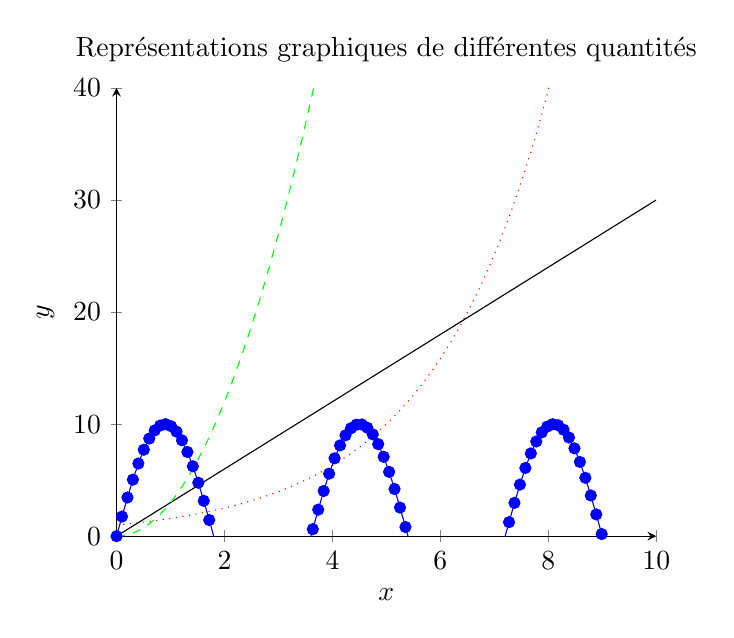
\begin{tikzpicture}
                  \begin{axis}[
                        title = {Représentations graphiques de différentes quantités},
                        axis lines = left,
                        xlabel = $x$,
                        %minor x tick num = 4,
                        ylabel = $y$,
                        ymin=0, ymax=40,
                        /pgf/number format/.cd,%3 lignes dessous, utiliser spacers français au lieu d'anglais.
                        use comma,
                        1000 sep={\,}
                      ]
                      %Below the red curve
                      \addplot [
                        domain=0:10,
                        samples=100,
                        color=red,
                        style=dotted
                        %/pgf/text mark = {+}, %changer le marqueur text
                        %mark=*,
                      ]
                      {10^(0.2*x)};
                      \addplot [
                        domain=0:10,
                        samples=100,
                        color=blue,
                        %/pgf/text mark = {+}, %changer le marqueur text
                        mark=*,
                      ]
                      {10*sin(100*x)};
                      \addplot [
                        domain=0:10,
                        samples=100,
                        color=black,
                        style=solid,
                        %/pgf/text mark = {+}, %changer le marqueur text
                        %mark=o,
                      ]
                      {3*x};
                      \addplot [
                        domain=0:10,
                        samples=100,
                        color=green,
                        style=dashed,
                        %/pgf/text mark = {+}, %changer le marqueur text
                        %mark=triangle,
                      ]
                      {3*x^2};
                  \end{axis}
              \end{tikzpicture}
             \end{figure}
        \end{question}
        \begin{reponses}
            \item[true] La courbe bleue (cercles).
		    \item[false] La courbe rouge (pointillés).
		    \item[false] La courbe noire (pleine).
		    \item[false] La courbe verte (tirets).
		    \end{reponses}
		    
		    
		     
			
		

		\subsection{Reconnaître les différentes représentations graphiques des fonctions usuelles}
		
			\begin{question}{30}{reconnaissance de courbes}{2}{}
            Parmi les différentes représentations de la figure suivante, laquelle représente une évolution exponentielle?
            \begin{figure}
              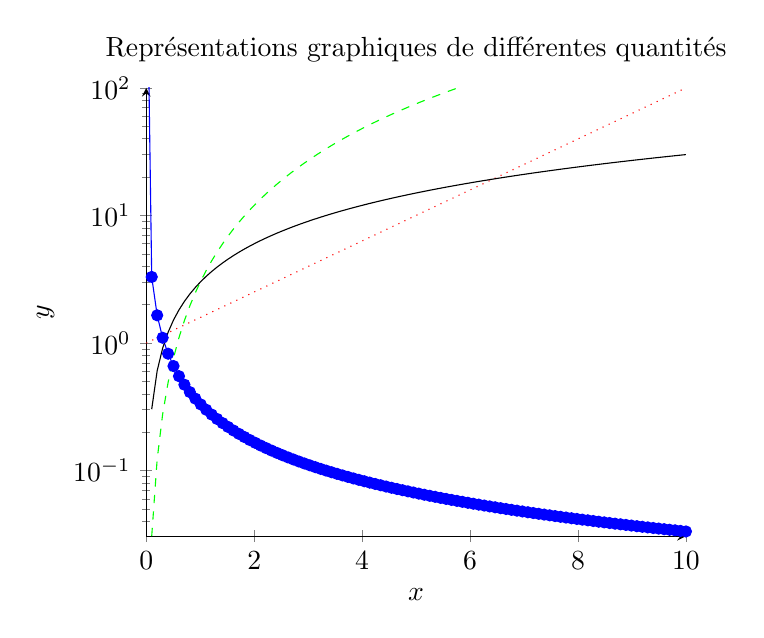
\begin{tikzpicture}
                  \begin{semilogyaxis}[
                        title = {Représentations graphiques de différentes quantités},
                        axis lines = left,
                        xlabel = $x$,
                        %minor x tick num = 4,
                        ylabel = $y$,
                        ymax=100,
                        /pgf/number format/.cd,%3 lignes dessous, utiliser spacers français au lieu d'anglais.
                        use comma,
                        1000 sep={\,}
                      ]
                      %Below the red curve
                      \addplot [
                        domain=0:10,
                        samples=100,
                        color=red,
                        style=dotted
                        %/pgf/text mark = {+}, %changer le marqueur text
                        %mark=o,
                      ]
                      {10^(0.2*x)};
                      \addplot [
                        domain=0.0001:10,
                        samples=100,
                        color=blue,
                        %/pgf/text mark = {+}, %changer le marqueur text
                        mark=*,
                      ]
                      {1/(3*x)};
                      \addplot [
                        domain=0:10,
                        samples=100,
                        color=black,
                        style=solid,
                        %/pgf/text mark = {+}, %changer le marqueur text
                        %mark=o,
                      ]
                      {3*x};
                      \addplot [
                        domain=0:10,
                        samples=100,
                        color=green,
                        style=dashed,
                        %/pgf/text mark = {+}, %changer le marqueur text
                        %mark=o,
                      ]
                      {3*x^2};
                  \end{semilogyaxis}
              \end{tikzpicture}
             \end{figure}
        \end{question}
        
        \begin{reponses}
            \item[false] La courbe bleue (cercles).
		    \item[true] La courbe rouge (pointillés).
		    \item[false] La courbe noire (pleine).
		    \item[false] La courbe verte (tirets).
		    \end{reponses}
        %%%%%%%%%%%%%%%%%%%%
        
        
         \begin{question}{N.A.}{reconnaissance de courbes}{1}{}
            Parmi les différentes représentations de la figure suivante, laquelle représente une évolution exponentielle?
            \begin{figure}
              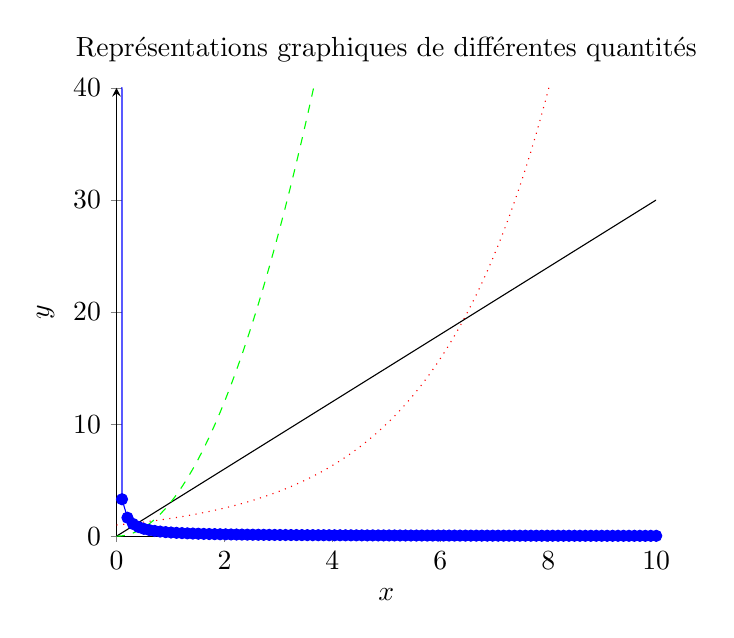
\begin{tikzpicture}
                  \begin{axis}[
                        title = {Représentations graphiques de différentes quantités},
                        axis lines = left,
                        xlabel = $x$,
                        %minor x tick num = 4,
                        ylabel = $y$,
                        ymin=0, ymax=40,
                        /pgf/number format/.cd,%3 lignes dessous, utiliser spacers français au lieu d'anglais.
                        use comma,
                        1000 sep={\,}
                      ]
                      %Below the red curve
                      \addplot [
                        domain=0:10,
                        samples=100,
                        color=red,
                        style=dotted
                        %/pgf/text mark = {+}, %changer le marqueur text
                        %mark=o,
                      ]
                      {10^(0.2*x)};
                      \addplot [
                        domain=0.0001:10,
                        samples=100,
                        color=blue,
                        mark=*,
                        %/pgf/text mark = {+}, %changer le marqueur text
                      ]
                      {1/(3*x)};
                      \addplot [
                        domain=0:10,
                        samples=100,
                        color=black,
                        %/pgf/text mark = {+}, %changer le marqueur text
                        %mark=o,
                        style=solid,
                      ]
                      {3*x};
                      \addplot [
                        domain=0:10,
                        samples=100,
                        color=green,
                        style=dashed,
                        %/pgf/text mark = {+}, %changer le marqueur text
                        %mark=o,
                      ]
                      {3*x^2};
                  \end{axis}
              \end{tikzpicture}
             \end{figure}
        \end{question}
        \begin{reponses}
            \item[false] La courbe bleue (cercles).
		    \item[true] La courbe rouge (pointillés).
		    \item[false] La courbe noire (pleine).
		    \item[false] La courbe verte (tirets).
		    \end{reponses}
        %%%%%%%%%%%%%%%%%%%%
        
        \begin{question}{NC}{reconnaissance de courbes}{2}{}
            Parmi les différentes courbes de la figure suivante, lesquelles représentent une évolution pseudo-périodique?
            \begin{figure}[!h]
              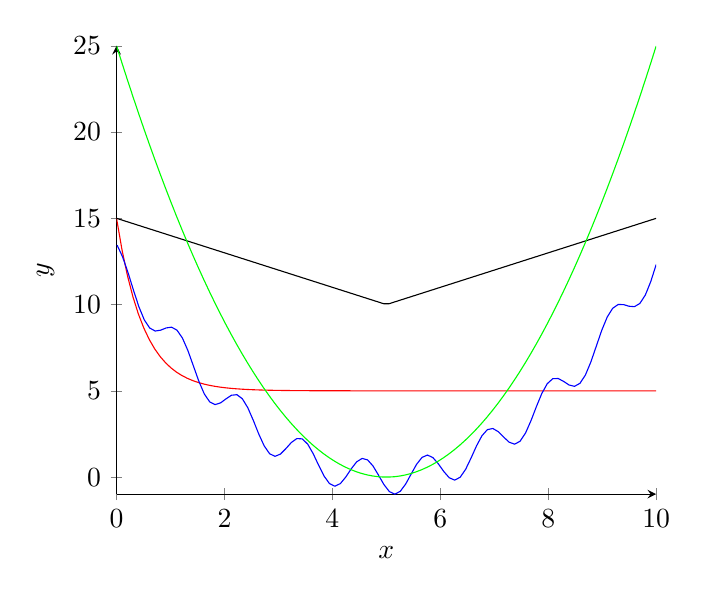
\begin{tikzpicture}
                  \begin{axis}[
                        title = { },
                        axis lines = left,
                        xlabel = $x$,
                        %minor x tick num = 4,
                        ylabel = $y$,
                        %ymin=0, ymax=40,
                        /pgf/number format/.cd,%3 lignes dessous, utiliser spacers français au lieu d'anglais.
                        use comma,
                        1000 sep={\,}
                      ]
                      %Below the red curve
                      \addplot [
                        domain=0:10,
                        samples=100,
                        color=red,
                        %/pgf/text mark = {+}, %changer le marqueur text
                        %mark=o,
                      ]
                      {10*exp(-2*x)+5};
                      \addplot [
                        domain=0.01:10,
                        samples=100,
                        color=blue,
                        %/pgf/text mark = {+}, %changer le marqueur text
                        %mark=o,
                      ]
                      {cos(2*3.14*50*x)+0.5*(x-5)^2};
                      \addplot [
                        domain=0:10,
                        samples=100,
                        color=black,
                        %/pgf/text mark = {+}, %changer le marqueur text
                        %mark=o,
                      ]
                      {abs(x-5)+10};
                      \addplot [
                        domain=0:10,
                        samples=100,
                        color=green,
                        %/pgf/text mark = {+}, %changer le marqueur text
                        %mark=o,
                      ]
                      {(x-5)^2};
                  \end{axis}
              \end{tikzpicture}
              \end{figure}
        \end{question}
        
        \begin{reponses}
            	\item[false]  La courbe noire
            	\item[false]   La courbe rouge
                \item[false]  La courbe verte
                \item[true]   La courbe bleue
            \end{reponses}
           %%%%%%%%%%%%%%%%%%%%%%%%%%%%%%%%%%%%%%%%%%%%%%%%%
           
           
              \begin{question}{N.A.}{reconnaissance de courbes}{2}{}
            Parmi les différentes représentations de la figure suivante, laquelle représente une évolution exponentielle?
            \begin{figure}
              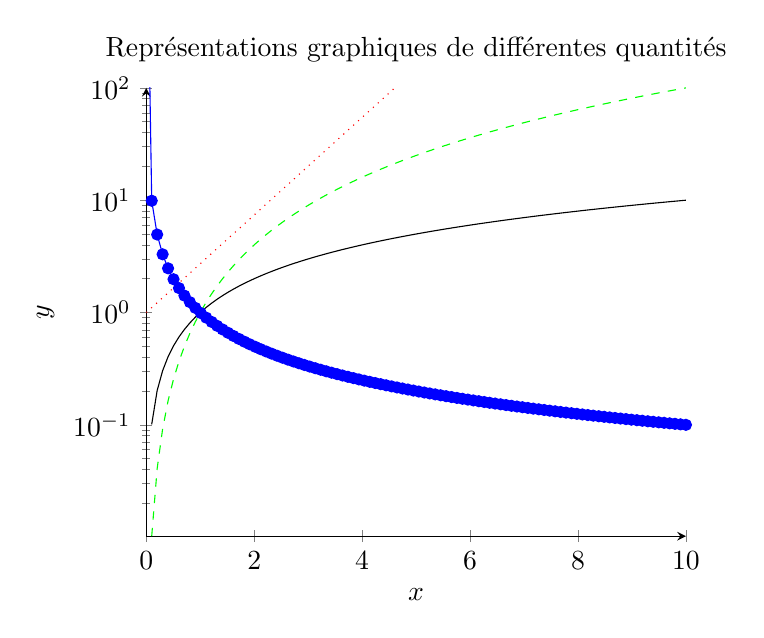
\begin{tikzpicture}
                  \begin{semilogyaxis}[
                        title = {Représentations graphiques de différentes quantités},
                        axis lines = left,
                        xlabel = $x$,
                        %minor x tick num = 4,
                        ylabel = $y$,
                        ymax=100,
                        /pgf/number format/.cd,%3 lignes dessous, utiliser spacers français au lieu d'anglais.
                        use comma,
                        1000 sep={\,}
                      ]
                      %Below the red curve
                      \addplot [
                        domain=0:10,
                        samples=100,
                        color=red,
                        style=dotted
                        %/pgf/text mark = {+}, %changer le marqueur text
                        %mark=o,
                      ]
                      {exp(x)};
                      \addplot [
                        domain=0.0001:10,
                        samples=100,
                        color=blue,
                        %/pgf/text mark = {+}, %changer le marqueur text
                        mark=*,
                      ]
                      {1/x};
                      \addplot [
                        domain=0:10,
                        samples=100,
                        color=black,
                        style=solid,
                        %/pgf/text mark = {+}, %changer le marqueur text
                        %mark=o,
                      ]
                      {x};
                      \addplot [
                        domain=0:10,
                        samples=100,
                        color=green,
                        style=dashed,
                        %/pgf/text mark = {+}, %changer le marqueur text
                        %mark=o,
                      ]
                      {x^2};
                  \end{semilogyaxis}
              \end{tikzpicture}
             \end{figure}
        \end{question}
        
        \begin{reponses}
            \item[false] La courbe bleue (cercles).
		    \item[true] La courbe rouge (pointillés).
		    \item[false] La courbe noire (pleine).
		    \item[false] La courbe verte (tirets).
		    \end{reponses}
        %%%%%%%%%%%%%%%%%%%%
        
        \begin{question}{N.A.}{reconnaissance de courbes}{2}{}
            Parmi les différentes représentations de la figure suivante, laquelle représente une évolution linéaire?
            \begin{figure}
              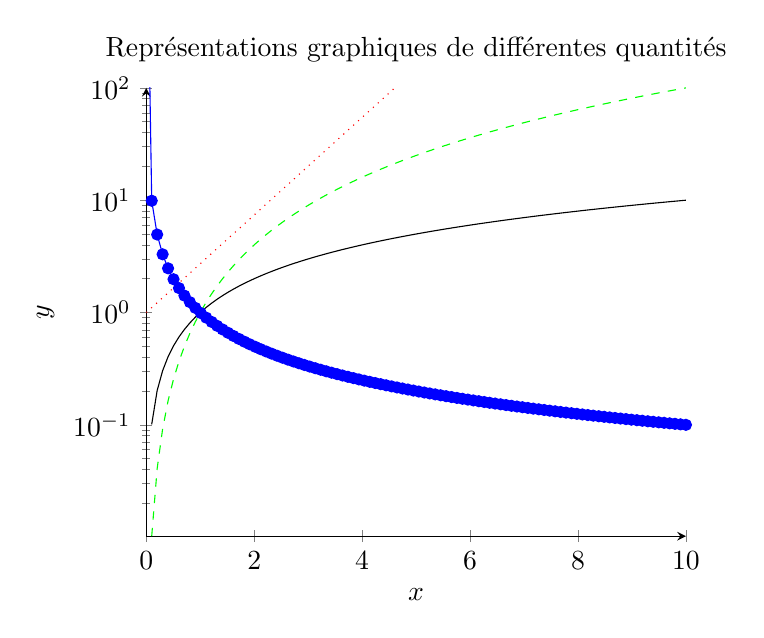
\begin{tikzpicture}
                  \begin{semilogyaxis}[
                        title = {Représentations graphiques de différentes quantités},
                        axis lines = left,
                        xlabel = $x$,
                        %minor x tick num = 4,
                        ylabel = $y$,
                        ymax=100,
                        /pgf/number format/.cd,%3 lignes dessous, utiliser spacers français au lieu d'anglais.
                        use comma,
                        1000 sep={\,}
                      ]
                      %Below the red curve
                      \addplot [
                        domain=0:10,
                        samples=100,
                        color=red,
                        style=dotted
                        %/pgf/text mark = {+}, %changer le marqueur text
                        %mark=o,
                      ]
                      {exp(x)};
                      \addplot [
                        domain=0.0001:10,
                        samples=100,
                        color=blue,
                        %/pgf/text mark = {+}, %changer le marqueur text
                        mark=*,
                      ]
                      {1/x};
                      \addplot [
                        domain=0:10,
                        samples=100,
                        color=black,
                        style=solid,
                        %/pgf/text mark = {+}, %changer le marqueur text
                        %mark=o,
                      ]
                      {x};
                      \addplot [
                        domain=0:10,
                        samples=100,
                        color=green,
                        style=dashed,
                        %/pgf/text mark = {+}, %changer le marqueur text
                        %mark=o,
                      ]
                      {x^2};
                  \end{semilogyaxis}
              \end{tikzpicture}
             \end{figure}
        \end{question}
        
        \begin{reponses}
            \item[false] La courbe bleue (cercles).
		    \item[false] La courbe rouge (pointillés).
		    \item[true] La courbe noire (pleine).
		    \item[false] La courbe verte (tirets).
		    \end{reponses}
        %%%%%%%%%%%%%%%%%%%%
        
        
        \begin{question}{N.A.}{reconnaissance de courbes}{3}{}
            On étudie l'évolution d'une population de bactérie au cours du temps. Soit N(t) le nombre de bactéries observées au temps t. N(t) est défini par la loi d'évolution suivante :$N_{cellules}=\frac{1000}{1+2exp(-2(t-3))}$. Parmi les différentes représentations de la figure suivante, laquelle représente l'évolution de N(t)?            
            \begin{figure}
              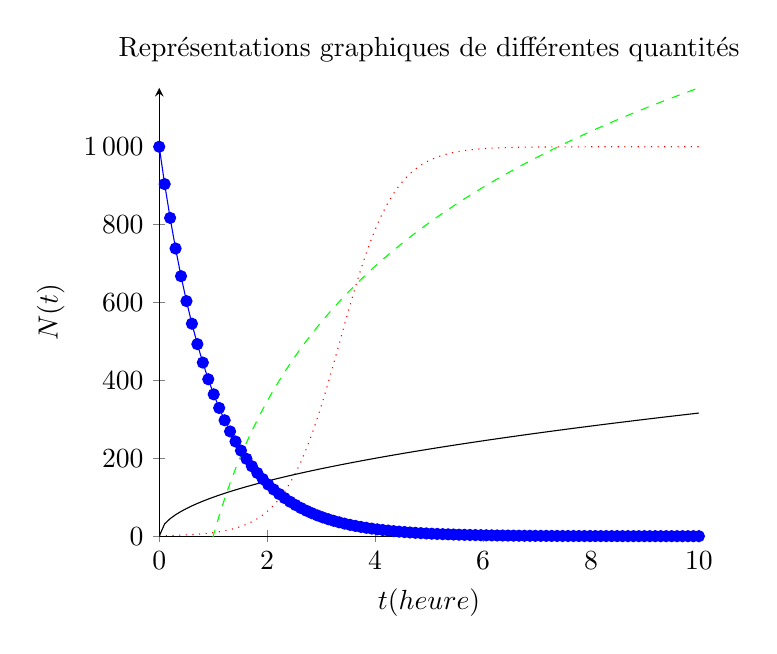
\begin{tikzpicture}
                  \begin{axis}[
                        title = {Représentations graphiques de différentes quantités},
                        axis lines = left,
                        xlabel = $t (heure)$,
                        %minor x tick num = 4,
                        ylabel = $N(t)$,
                        ymin=0,
                        /pgf/number format/.cd,%3 lignes dessous, utiliser spacers français au lieu d'anglais.
                        use comma,
                        1000 sep={\,}
                      ]
                      %Below the red curve
                      \addplot [
                        domain=0:10,
                        samples=100,
                        color=red,
                        style=dotted
                        %/pgf/text mark = {+}, %changer le marqueur text
                        %mark=o,
                      ]
			          {1000/(1+2*exp(-2*(x-3)))};
                      \addplot [
                        domain=0:10,
                        samples=100,
                        color=blue,
                        %/pgf/text mark = {+}, %changer le marqueur text
                        mark=*,
                      ]
                      {1000*exp(-x)};
                      \addplot [
                        domain=0:10,
                        samples=100,
                        color=black,
                        style=solid,
                        %/pgf/text mark = {+}, %changer le marqueur text
                        %mark=o,
                      ]
                      {100*sqrt(x)};
                      \addplot [
                        domain=0:10,
                        samples=100,
                        color=green,
                        style=dashed,
                        %/pgf/text mark = {+}, %changer le marqueur text
                        %mark=o,
                      ]
                      {500*ln(x)};
                  \end{axis}
              \end{tikzpicture}
             \end{figure}
        \end{question}
        
        \begin{reponses}
            \item[false] La courbe bleue (cercles).
		    \item[true] La courbe rouge (pointillés).
		    \item[false] La courbe noire (pleine).
		    \item[false] La courbe verte (tirets).
		    \end{reponses}
        %%%%%%%%%%%%%%%%%%%%
         
            \begin{question}{30}{Fonctions usuelles}{2}{/}
            On étudie l'évolution d'une population de bactérie au cours du temps. Soit N(t) le nombre de bactéries observées au temps t. N(t) est défini par la loi d'évolution suivante : $N(t) = 10\exp{-2t}$. Parmi les différentes représentations de la figure suivante, laquelle représente l'évolution de N(t)?            \begin{figure}
              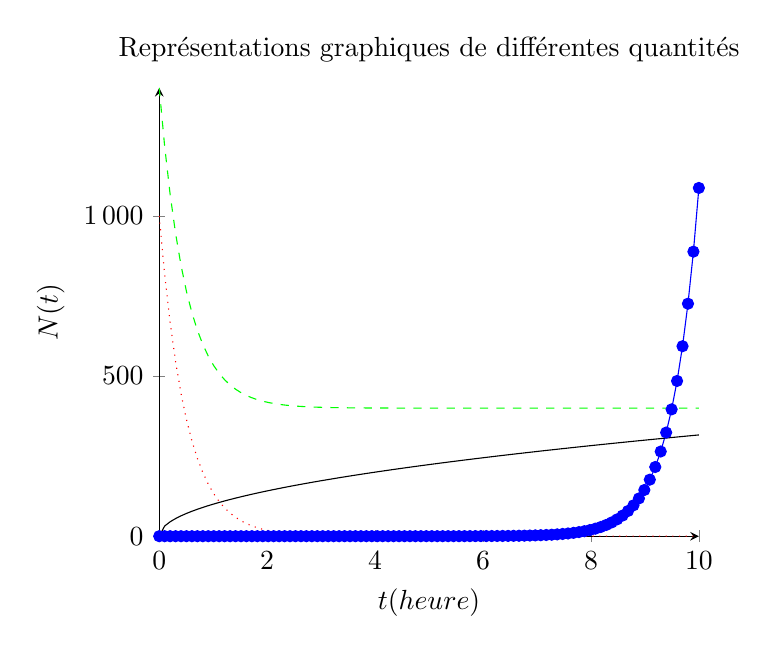
\begin{tikzpicture}
                  \begin{axis}[
                        title = {Représentations graphiques de différentes quantités},
                        axis lines = left,
                        xlabel = $t (heure)$,
                        %minor x tick num = 4,
                        ylabel = $N(t)$,
                        %ymax=100,
                        /pgf/number format/.cd,%3 lignes dessous, utiliser spacers français au lieu d'anglais.
                        use comma,
                        1000 sep={\,}
                      ]
                      %Below the red curve
                      \addplot [
                        domain=0:10,
                        samples=100,
                        color=red,
                        style=dotted
                        %/pgf/text mark = {+}, %changer le marqueur text
                        %mark=o,
                      ]
                      {1000*exp(-2*x)};
                      \addplot [
                        domain=0:10,
                        samples=100,
                        color=blue,
                        %/pgf/text mark = {+}, %changer le marqueur text
                        mark=*,
                      ]
                      {1e-3*exp(2*x-5)/3};
                      \addplot [
                        domain=0:10,
                        samples=100,
                        color=black,
                        style=solid,
                        %/pgf/text mark = {+}, %changer le marqueur text
                        %mark=o,
                      ]
                      {sqrt(x)*100};
                      \addplot [
                        domain=0:10,
                        samples=100,
                        color=green,
                        style=dashed,
                        %/pgf/text mark = {+}, %changer le marqueur text
                        %mark=o,
                      ]
                      {1000*exp(-2*x)+400};
                  \end{axis}
              \end{tikzpicture}
             \end{figure}
        \end{question}
        
        \begin{reponses}
            \item[false] La courbe bleue (cercles).
		    \item[true] La courbe rouge (pointillés).
		    \item[false] La courbe noire (pleine).
		    \item[false] La courbe verte (tirets).
		    \end{reponses}
        %%%%%%%%%%%%%%%%%%%%
        
      
	    \subsection{Mise en application: Spectrophotométrie}

            \begin{question}{NC}{Beer-Lambert}{1}{/} 
				La loi de Beer-Lambert est une relation empirique reliant l'atténuation de la lumière aux propriétés du milieu qu'elle traverse et à l'épaisseur traversée. Cette loi est très utilisée pour connaître la concentration d'une solution. Elle s'exprime de la manière suivante : $A=\epsilon C l$ avec $A$ l'absorbance (ou densité optique), $\epsilon$ le coefficient d'absorption molaire en $\si{\liter\per\mole\per\centi\meter}$, $C$ la concentration de la solution en $\si{\mole\per\liter}$ et $l$ la largueur de la cuve mise dans le spectrophotomètre en $\si{\centi\meter}$. Mais au fait, que nous dit la loi de Beer-Lambert concernant la relation entre la concentration C de la solution étudiée, et l'absorbance (ou densité optique) A ? 

            \end{question}

            \begin{reponses}
            	\item[false]  Elle est parabolique
            	\item[true]   Elle est linéaire
                \item[false]  Elle est exponentielle
                \item[false]  Elle est logarithmique
            \end{reponses}
			%%%%%%%%%%%%%%%%%%%%%%%%%%%%%%%%%%%%%
            
            \begin{question}{NC}{Beer-Lambert}{2}{/} 
				On dispose d'une solution aqueuse contenant des ions $Cu^{2+}$, de concentration $C_0= \SI{ 5,0e-2}{\mol\per\liter}$. On mesure son spectre grâce à un spectrophotomètre et en plaçant cette solution dans une cuve de largeur $l= \SI{1,0}{\si\centi\meter}$. L'espèce $Cu^{2+}$ est colorée. On mesure la valeur d'absorbance maximale pour la solution étudiée et on trouve $A_{max} = 0.43$. En déduire le coefficient d’absorption molaire de la solution en $Cu^{2+}$,noté $\epsilon_{Cu}$, à la longueur d’onde $\lambda_m$ pour laquelle l’absorbance est maximale.

            \end{question}
%
           \begin{reponses}
            	\item[true] $\epsilon_{Cu} =  \SI{8.6}{\liter\per\mole\per\centi\meter}$
            	\item[false] $\epsilon_{Cu} = \SI{0.86}{\liter\per\mole\per\centi\meter}$
                \item[false] $\epsilon_{Cu} = \SI{7.5}{\liter\per\mole\per\centi\meter}$
                \item[false] $\epsilon_{Cu} = \SI{0.75}{\liter\per\mole\per\centi\meter}$
                \item[false] $\epsilon_{Cu} = \SI{0.21}{\liter\per\mole\per\centi\meter}$
            \end{reponses}
			%%%%%%%%%%%%%%%%%%%%%%%%%%%%%%%%%%%%%
			
			\begin{question}{1221}{calcul de limite}{2}{/}
			\begin{figure}
                \begin{tikzpicture}
        		\begin{axis}[
                    title = ,
                    xlabel ={temps (h)},
                    ylabel ={$N_{cellules}$},]
                    % density of Normal distribution:
        			\addplot [
                      red,
                      domain =0:200,
                      samples =201,
             		]
        			  {200*exp(-0.02*x)+100/(1+2*exp(-0.02*(x-100)))};
        		\end{axis}
        		\end{tikzpicture}
        		\end{figure}
                La figure ci-dessus représente l'évolution d'une population de cellules en fonction du temps. Voici l'expression du nombre de cellules $N_{cellules}$ en fonction du temps : $N_{cellules}= 200\exp(-0.02t)+\frac{100}{1+2exp(-0.02(t-100))}$. Pour un temps très grand, quel sera le nombre de cellules observées ? 
            \end{question}     

				\begin{reponses}
            	\item[false]  $0 $ 
            	\item[true]   $100 $ 
                \item[false]   $+\infty $ 
                \item[false]  $150 $ 
                
                \end{reponses}
		
			
        	\begin{question}{1221}{Fonctions usuelles}{2}{/}
				Une société produit des bactéries pour l’industrie. En laboratoire, on mesure, dans un milieu nutritif approprié, la masse de ces bactéries, mesurée en grammes. On note $M(t)$ la masse mesurée, en kilogramme, au cours du temps $t$ en jours. L'évolution de la masse mesurée au cours du temps est définie par la fonction suivante : $M(t) = \frac{50}{1+49\exp{-0.2t}}$. Au bout d'un très grand ($t \to +\infty$), vers quoi va tendre la masse mesurée ?
%enunjour.
            \end{question}

            \begin{reponses}
            	\item[false] $+\infty$
            	\item[false] $\SI{0}{\kilo\gram}$
                \item[false] $\SI{1}{\kilo\gram}$
                \item[true] $\SI{50}{\kilo\gram}$
            \end{reponses}
			%%%%%%%%%%%%%%%%%%%%%%%%%%%%%%%%%%%%%

%--------
    \section{Calcul}
    
        \subsection{Changer d'unités}
        
            \begin{question}{}{Unités}{1}{}
                À quoi correspond un \si{ppm} (partie par million)?
            \end{question}
                
            \begin{reponses} 
                \item[false] \SI{1e-4}{\percent}
                \item[false] \SI{0.01}{\percent}
                \item[true] \num{1e-6}
        	    \item[false] \SI{100}{\percent}
            \end{reponses}
            
            
            
            \begin{question}{}{Unités}{2}{}
                On mesure la concentration d'un soluté dans une solution en g/L. Lorsque les quantités de soluté sont très petites dans une grande quantité de solution, on mesure plutôt la concentration en ppm (Parties Par Millions).La concentration en ppm se mesure en g de soluté par millions de grammes de solution, soit g/Mg.
                1 ppm = 1g (de soluté)/1 000 000 g (de solution) ou encore  1 ppm = 1g (de soluté)/1 000 000 mL (de solution) 
                
                On a mesuré la quantité de polluants émis dans l'eau au bord d'un lac. Sur 250 L d'eau prélevés, on retrouve 45 mg de polluants. Quelle est la concentration de polluants en ppm au bord du lac? 
            \end{question}
              
            \begin{reponses} 
                \item[true]   \SI{.18}{ppm}
                \item[false]  \SI{.25}{ppm}
                \item[false]   \SI{1.8}{ppm}
        	    \item[false]  \SI{2.3}{ppm}
            \end{reponses}
            
            \begin{question}{}{Unités}{2}{}
                \frquotes{ppm} signifiant \frquotes{parties par million}, est une unité utilisée pour indiquer le nombre d'atomes ou molécules d'un certain soluté présents dans une solution données. Par exemple, dire que l'on a \SI{20}{ppm} de di-oxygène dans un verre d'eau signifie que pour un million de molécules prises au hasard dans ce verre, 20 seront des molécules de di-oxygène.\\
                Quel est le volume d'une solution contenant \SI{50.00}{ppm} de \SI{18}{\gram} de soluté. 
            \end{question}
              
            \begin{reponses} 
                \item[true]   \SI{360}{\liter}
                \item[false]  \SI{36.0}{\liter}
                \item[false]   \SI{3.6}{\liter}
        	    \item[false]  \SI{0.36}{\liter}
            \end{reponses}
    
        \subsection{Mise en application : Biologie-Chimie (proportionnalité)}

            \begin{question}{1215}{dilution}{1}{}
                Lors d'une dilution, pour faire une solution fille de concentration $C_f$ et de volume $V_f$ à partir d'une solution mère concentration molaire $C_m$, on prélève un volume $V_m$ de la solution mère que l'on dilue. Quelle est relation reliant la concentration des solutions mère et fille au volume prélevé de la solution mère et au volume de la solution fille ?
            \end{question}
            \begin{reponses}
                \item[true] $C_f\cdot V_f = C_m\cdot V_m$
                \item[false] $C_f\cdot V_m = C_m\cdot V_f$
                \item[false] $C_f/V_f = C_m/V_m$
        	    \item[false] $V_f/C_f = V_m/C_m$
            \end{reponses}
            %%%%%%%%%%%%%%%%%%%%
            
            \begin{question}{1215}{Chimie}{1}{/}
    			 Soit $N$ le nombre d'entités chimiques contenu dans un échantillon. Que vaut $N$ en fonction de  $n$, le nombre de moles dans cet échantillon, et le nombre d'Avogadro $N_a$, qui correspond au facteur de conversion entre le gramme et l'unité de masse atomique. 
            \end{question}

            \begin{reponses}
            	\item[false] $ \frac{n}{N_a} $
            	\item[false] $ n^{N_a}$
                \item[true]  $ n.N_a $
                \item[false] $ \frac{N_a}{n} $
            \end{reponses}
			%%%%%%%%%%%%%%%%%%%%%%%%%%%%%%%%%%%%%
			
		
		    \begin{question}{1210}{calcul}{2}{/}
				  Combien y a-t-il de moles d'eau $n$ dans un litre d'eau ? (info : $M(H) =1,0\ g.mol^{-1}$ ;  $M(O) = 16,0\ g.mol^{-1}$)

            \end{question}

            \begin{reponses}
            	\item[false] $\SI{6.25e1}{\mol} $
            	\item[true]  $ \SI{5.55e1}{\mol} $
                \item[false] $ \SI{5.55e-1}{\mol} $
                \item[false] $ \SI{6.25e-1}{\mol} $
            \end{reponses}
			%%%%%%%%%%%%%%%%%%%%%%%%%%%%%%%%%%%%%
			
			
			\begin{question}{1210}{calcul}{3}{/}
				  Les bactéries se reproduisent par division binaire, phase de division de durée fixe que nous appellerons période. On note $P_n$ la population au bout de n périodes de reproduction, avec $n \in \NN $. On peut montrer que le nombre de bactéries au cycle n est défini par $P_n = 2^n$. Sachant que $\forall (a,x) \in \RR, ln(a^x) = x\ln{a}$, trouver à partir de quel cycle le nombre de bactéries dépasse $10^6$. 

            \end{question}

            \begin{reponses}
            	\item[false] 15
            	\item[false] 8
                \item[true]  20
                \item[false] 50
            \end{reponses}
			%%%%%%%%%%%%%%%%%%%%%%%%%%%%%%%%%%%%%
		    
			\begin{question}{1210}{calcul}{2}{/}
				 A partir d’une solution mère de S on prépare une solution fille S' en prélevant un volume $V = \SI{350}{\micro\liter}$ de la solution mère et en rajoutant certain volume d’eau. Le volume $V'$ de la solution fille vaut $V' = \SI{100}{\milli\liter}$. Que vaut le facteur de dilution FD ? (c'est-à-dire : Combien de fois a-t-on dilué la solution mère ?) 
                 

            \end{question}

            \begin{reponses}
            	\item[false]  $\SI{2.86e-3}{} $
            	\item[false]  $ \SI{3.50e-6}{}$
                \item[false]  $ \SI{2.86e2}{}$
                \item[true]   $ \SI{3.50e-3}{}$
            \end{reponses}
			%%%%%%%%%%%%%%%%%%%%%%%%%%%%%%%%%%%%%
			
			
	
             \begin{question}{}{dilution}{2}{1215,1209,1210,1211}
				 A partir d’une solution mère de $H_2SO_4$ « 1M »  (concentration $C_{mere} = \SI{1} {\mole\per\liter}$), vous devez préparer $\SI{500}{\milli\liter}$ de $H_2SO_4$ « 50mM » (concentration $C_{fille} = 50 \si{\milli\mole\per\liter}$). Quel volume de solution mère doit être prélevé?  (En pratique, ce volume sera rajouté à un volume d'eau pour avoir le volume de solution désiré).
            \end{question}

            \begin{reponses}
            	\item[true]  $\SI{25}{\milli\liter} $
            	\item[false]  $ \SI{25e-2}{\liter} $
                \item[false]   $ \SI{250}{\milli\liter} $
                \item[false]  $ \SI{0.25}{\milli\liter} $
            \end{reponses}
			%%%%%%%%%%%%%%%%%%%%%%%%%%%%%%%%%%%%%
        

        	\begin{question}{1210}{Grandeurs chimiques}{1}{/}
				On considère une solution de concentration molaire $C$ et de volume $V$. Exprimer $C$ en fonction de la quantité de moles $n$ dans la solution et de  $V$. 
            \end{question}

            \begin{reponses}
            	\item[true]  $\frac{n}{V}$
            	\item[false] $ n V$
                \item[false] $ \frac{V}{n}$
                \item[false] $ n^{V}$
            \end{reponses}
			%%%%%%%%%%%%%%%%%%%%%%%%%%%%%%%%%%%%%
            
            \begin{question}{1210}{Grandeurs chimiques}{2}{/}
				Soit une masse $m$ de sel que l'on dilue dans $\SI{5}{\deci\liter}$ d'eau. Sachant que la concentration massique $C_m$ de sel dissout dans l'eau est de $\SI{3e-2}{\gram\per\liter}$, quelle est la masse de sel initiale ?  
            \end{question}

            \begin{reponses}
            	\item[false] $\SI{15}{\gram}$
            	\item[false] $\SI{6e-2}{\gram}$
                \item[false] $\SI{1,6e-1}{\gram}$
                \item[true]  $\SI{15e-3}{\gram}$
            \end{reponses}
			%%%%%%%%%%%%%%%%%%%%%%%%%%%%%%%%%%%%%
            
            \begin{question}{1210}{Grandeurs chimiques}{2}{/}
				  Vous devez préparer \SI{150}{mL} de gel à \SI{1.2}{\percent} d’agarose. Un produit dosé à Y \% signifie qu'il a Y grammes de produit actif pour 100 ml. Quelle quantité $m$ d’agarose devez-vous peser ?

            \end{question}

            \begin{reponses}
            	\item[true]  \SI{1.8}{\gram}
            	\item[false]  \SI{8e-5}{\gram}
                \item[false]  \SI{0.3}{\milli\gram}
                \item[false]   \SI{2e-2}{\milli\gram}
            \end{reponses}
			%%%%%%%%%%%%%%%%%%%%%%%%%%%%%%%%%%%%%
			
			
			
			\begin{question}{1210}{proportionalité}{2}{/}
		        Les bactéries Escherichia Coli se reproduisent par division binaire, phase de division de durée fixe que nous appellerons période. On note $P_n$ la population au bout de n périodes de reproduction, avec $n \in \NN $. On peut montrer que le nombre de bactéries au cycle n est défini par $P_n = 2^n$. Pour 24 heures, ce qui représentent 72 périodes de reproduction, nous aurions une population de $2^{72} = 4,72.10^{21}$ bactéries. La masse d’une bactérie étant d’environ $\SI{7e-13}{\gram}$, quelle sera la masse obtenue au bout de 24 heures ? 

            \end{question}

            \begin{reponses}
            	\item[false]  $ \SI{1457}{\kilo\gram} $
            	\item[false]  $ \SI{2.45}{\giga\tonne} $
                \item[true]  $ \SI{1170}{\tonne} $
                \item[false]   $ \SI{5,97e24}{\kilo\gram} $
            \end{reponses}
			%%%%%%%%%%%%%%%%%%%%%%%%%%%%%%%%%%%%%
			
			\begin{question}{1210}{Calcul}{2}{/}
				 A partir d’une solution mère de S on prépare une solution fille S' en prélevant un volume $V = \SI{350}{\micro\liter}$ de la solution mère et en rajoutant un certain volume de solution tampon. Le volume $V'$ de la solution fille vaut $V' = \SI{100}{\milli\liter}$. Combien de fois a-t-on dilué la solution mère ? (i.e quel est le facteur de dilution FD ? ) 
                 

            \end{question}

            \begin{reponses}
            	\item[false]  $FD = \SI{2.86e-3}{} $
            	\item[false]  $FD = \SI{3.50e-6}{}$
                \item[false]  $FD = \SI{2.86e2}{}$
                \item[true]   $FD = \SI{3.50e-3}{}$
            \end{reponses}
			%%%%%%%%%%%%%%%%%%%%%%%%%%%%%%%%%%%%%

      
			
			\begin{question}{1216,8,1209}{Calcul de concentration}{2}{}
				Les antibiotiques sont des molécules possédant la propriété de tuer des bactéries ou d'en limiter la propagation. La concentration dans le sang, en $\si{\milli\gram\per\liter}$, en fonction du temps d'un antibiotique injecté en une seule prise à un patient est défini par la fonction suivante $g(t) = \frac{4t}{t^{2}+1}$. t est le temps en heure. Au bout de combien d'heures, la concentration en antibiotique dans le sang vaut \SI{2}{\milli\gram\per\liter}  ?

            \end{question}

            \begin{reponses}
            	\item[true] 1 heure
            	\item[false]  2 heures
                \item[false]  3 heures
                \item[false] 4  heures
            \end{reponses}
			%%%%%%%%%%%%%%%%%%%%%%%%%%%%%%%%%%%%%
			
				\begin{question}{1216}{Calcul}{2}{1215}
                On étudie l'évolution d'une population de bactéries présentent dans une boite de Pétri. À $t=\SI{0}{\hour}$, on en compte \num{1500}. Au bout de \SI{2}{\hour}, leur nombre a été augmenté de \SI{120}{\percent}. Combien compte-t-on de bactéries à $t=\SI{2}{\hour}$?
            \end{question}

            \begin{reponses}
            	\item[false] \num{181500}
            	\item[true]  \num{3300}
                \item[false]  \num{1800}
                \item[false] \num{1262}
            \end{reponses}
			%%%%%%%%%%%%%%%%%%%%%%%%%%%%%%%%%%%%%
			
			
			\begin{question}{1216}{Calcul}{3}{1215}
                On étudie l'évolution d'une population de bactéries présentent dans une boite de Pétri. À $t=\SI{0}{\hour}$, on en compte \num{1000}. Au bout de \SI{2}{\hour}, on en compte \num{3000}. De combien à augmenté le nombre de bactéries? 
            \end{question}

            \begin{reponses}
            	\item[false] \SI{300}{\percent}
            	\item[true]  \SI{200}{\percent}
                \item[false] \SI{100}{\percent}
                \item[false] \SI{600}{\percent}
            \end{reponses}
			%%%%%%%%%%%%%%%%%%%%%%%%%%%%%%%%%%%%%
        
       

         \begin{question}{60,61,1214}{BIo}{3}{}
          On s'intéresse à l'évolution d'une population de bactéries en fonction du temps. Soit N(t) le nombre de bactérie au temps t défini par l'expression suivante : $N(t) = (x^2+3)^2 $. Calculer le nombre de bactéries observées entre le début de l'expérience (t=0h) et la fin de l'expérience (t=10h), c'est à dire calculer $\int^{10}_{0} N(t) \mathrm{d}t$.
        \end{question}
        \begin{reponses}
            \item[false] $12568$
            \item[true] $22090$
            \item[false]  $+\infty$
            \item[false] $-12568$
        \end{reponses}
        %%%%%%%%%%%%%%%%%%%%
			

            \begin{question}{8}{équations}{2}{/} 
            	Pour savoir si une expérience est compatible avec le modèle théorique utilisé, on utilise l'erreur relative $\delta = \frac{|theorie-experience|}{theorie}$. Sur une population de 300 mouches, on compte le nombre de mouches aux yeux rouges. Si on considère qu'un seul gène est à l'origine de la couleur des yeux, on estime à 3/4 le ratio entre le nombre de mouches rouges aux yeux rouges et le nombre total de mouches. Sachant que l'erreur relative calculée est de $6.6\%$, quel est le nombre de mouches aux yeux rouges comptés ? 
            \end{question}

            \begin{reponses}
            	\item[false]  150
            	\item[false]  50
                \item[false]  250
                \item[true]   210
            \end{reponses}
			%%%%%%%%%%%%%%%%%%%%%%%%%%%%%%%%%%%%%
	

	

			\section{Statistiques}
			
			  \subsection{généralités}

            \begin{question}{NC}{Stats}{1}{/} 
				En biologie ou en physique, il est important de savoir utiliser les outils mathématiques que sont les statistiques pour mener à bien nos expériences. Un concept important est celui de la variance d'une distribution/d'un échantillon statistique. Qu'est-ce que la variance ? 

            \end{question}

            \begin{reponses}
            	\item[false]  Elle permet de déduire la variation dans le temps de notre distribution
            	\item[false]  Elle permet de mesurer la taille de l'échantillon 
                \item[false]  Elle indique si nos données sont fausses
                \item[true]   Elle permet de mesurer la dispersion des points autour de la valeur moyenne 
            \end{reponses}
			%%%%%%%%%%%%%%%%%%%%%%%%%%%%%%%%%%%%%
            
            

            
            
            \begin{question}{NC}{Proba}{1}{/} 
				Jouer à pile ou face est une situation assez simple dans laquelle à chaque essai on a une probabilité $p$ de gagner (si pile équivaut à un succès) et $(1-p)$ de perdre (si face équivaut à un échec). Cette situation assez binaire est décrite par la loi de Bernoulli ou loi Binomiale $B(n,p)$ qui permet de calculer la probabilité d'obtenir k succès en n tentatives (c'est-à-dire $P(X=k)$, avec $X$ une variable aléatoire ), avec une probabilité $p$ d'obtenir un succés à chaque tentative. Certaines situations dans la nature peuvent également être décrites par une loi binomiale : avoir les yeux rouges ou blancs pour les mouches par exemple. Exprimer la probabilité $P(X=k)$ donnée par la loi binomiale.

            \end{question}

            \begin{reponses}
            	\item[true]   $ \binom{n}{k}p^{k}(1-p)^{n-k}$
            	\item[false]  $  p^{k}(1-p)^{n-k}$
                \item[false]  $  \binom{n+k}{k}p^{k}(1-p)^{n-k}$
                \item[false]  $  p^{k}$
            \end{reponses}
			%%%%%%%%%%%%%%%%%%%%%%%%%%%%%%%%%%%%%
            
            
            \begin{question}{NC}{Proba}{2}{/} 
 				En supposant que l'apparition des yeux rouges est dû à un seul gène dominant, on peut établir que le nombre de descendants F2 aux yeux rouges dans un échantillon de 200 mouches suit une loi binomiale $B(200,3/4)$. Sachant que la probabilité de trouver au moins 149 mouches aux yeux rouges vaut 0.462, calculer la probabilité de trouver au moins 150 mouches au yeux rouges.
            \end{question}

            \begin{reponses}
            	\item[false] $0.785$
            	\item[false] $1.245$
                \item[false] $0.245$
                \item[true]  $0.537$
            \end{reponses}
			%%%%%%%%%%%%%%%%%%%%%%%%%%%%%%%%%%%%%
            
            
             \begin{question}{NC}{Proba}{2}{/} 
 				On croise une souche de drosophiles aux yeux rouges, avec une souche de drosophiles aux yeux blancs. Tous les hybrides F1 ont les yeux rouges. On croise les hybrides F1 entre eux et on observe à la loupe binoculaire la couleur des yeux de 200 descendants F2. On trouve 60 mouches aux yeux blancs, et 140 mouches aux yeux rouges. Quelle est la proportion de mouches aux yeux rouges dans la descendance F2?
            \end{question}

            \begin{reponses}
            	\item[false]  $75\%$
            	\item[true]   $70\%$
                \item[false]  $30\%$
                \item[false]  $25\%$
            \end{reponses}
			%%%%%%%%%%%%%%%%%%%%%%%%%%%%%%%%%%%%%
			
			
			
			\begin{question}{NC}{Stats}{1}{/} 
			\includegraphics[width=\textwidth]{Christopher/Figures_Christopher/glycemie_UE.png}
				La figure ci-dessus montre sous forme d’histogrammes le résultat d’une étude visant à mesurer la glycémie à jeun auprès de 100 patients «sains», et 100 patients diabétiques d’un hopital. Choisir les bonnes réponses

            \end{question}

            \begin{reponses}
            	\item[true]  La variance du groupe "sains" est plus élevée que celle du groupe "diabétiques"
            	\item[false] La moyenne du groupe "diabétiques" est plus élevée que celle du groupe "sains"
                \item[true]  La variance du groupe "sains" est inférieure à celle du groupe "diabétiques"
                \item[false] La moyenne du groupe "diabétiques"  est inférieure à celle du groupe "diabétiques"
            \end{reponses}
			%%%%%%%%%%%%%%%%%%%%%%%%%%%%%%%%%%%%%
			
			
			
			 \begin{question}{NC}{Proba}{1}{/} 
 				Dans une expérience, le physicien ou le biologiste manipule la plupart du temps plusieurs variables/paramètres. Il est donc important d'utiliser les outils mathématiques pour savoir si ces paramètres ont un lien entre eux ou non. Pour ce faire on utilise le facteur de corrélation $\rho$, avec $\rho\in [-1,1]$. Cet outil permet de déterminer s'il existe une relation linéaire entre deux paramètres $A$ et $B$. Parmi les situations suivantes, choisir les bonnes propositions: 

            \end{question}

            \begin{reponses}
            	\item[true]  Si $A$ et $B$ sont indépendants, alors $\rho =0 $.
            	\item[false] Si $\rho =0 $, alors $A$ et $B$ sont indépendants.
                \item[true]  Si $\rho \simeq 1 $, alors $A$ et $B$ sont dépendants.
                \item[false] Si $\rho \simeq -1 $, alors $A$ et $B$ sont indépendants.
            \end{reponses}
			%%%%%%%%%%%%%%%%%%%%%%%%%%%%%%%%%%%%%
			
			
			\begin{question}{NC}{Proba}{2}{/} 
            \includegraphics[width=\textwidth]{Christopher/Figures_Christopher/correlation_UE.png}
 				Deux grandeurs (notées X et Y) sont mesurées dans deux groupes d’individus. Les graphes sont donnés ci-dessus. Ces deux groupes ont conduit au calcul de deux coefficients de corrélation égaux à 0,9 et 0. Choisir les bonnes propositions : 

            \end{question}

            \begin{reponses}
            	\item[true]  La corrélation est nulle pour A et de 0,9 pour B
            	\item[false] La corrélation est de 0,9 pour A et nulle pour B
                \item[true]  Les deux mesures X et Y sont indépendantes pour A
                \item[false] Les deux mesures X et Y sont indépendantes pour B
            \end{reponses}
			%%%%%%%%%%%%%%%%%%%%%%%%%%%%%%%%%%%%%


    \section{Vecteurs}
        \subsection{Savoir ce qu'est un vecteur}
        
        	\begin{question}{non créé}{Vecteurs}{1}{/}
				Soit $\vec{A}$ un vecteur en deux dimensions. Sa coordonnée sur l'axe $x$ est $a_x$, et sa coordonnée sur l'axe $y$ est $a_y$. Lesquelles de ces quantité est égale à $\vec{A}$?
            \end{question}

            \begin{reponses}
            	\item[false] $(a_x+a_y;a_x-a_y)$
            	\item[true] $a_x\vec{u_x}+a_y\vec{u_y}$ où $\vec{u_x}$ et $\vec{u_y}$ sont les vecteurs unitaires des axes $x$ et $y$
                \item[false] $\sqrt{a_{x}^2+a_{y}^2}$
                \item[false] $(\sqrt{a_{x}^2+a_{y}^2};\sqrt{a_{x}^2-a_{y}^2})$
            \end{reponses}
			%%%%%%%%%%%%%%%%%%%%%%%%%%%%%%%%%%%%%

        \subsection{Calculer la norme d'un vecteur}
        
        	\begin{question}{1202}{Vecteurs}{1}{/}
				Soit un vecteur $\vec{A}$ de coordonnées $(a_x;a_y)$. Quelle est la norme de ce vecteur?
            \end{question}

            \begin{reponses}
            	\item[false] $a_x+a_y$
            	\item[false] $a_x\times a_y$
                \item[false] $a_{x}^2+a_{y}^2$
                \item[true] $\sqrt{a_{x}^2+a_{y}^2}$
            \end{reponses}
			%%%%%%%%%%%%%%%%%%%%%%%%%%%%%%%%%%%%%
			
			 \subsection{Déterminer les composantes d'un vecteur dans un repère orthonormé à partir des coordonnées des points de départ et d'arrivée}
        
        	\begin{question}{1201}{Vecteurs}{1}{1220}
				Dans un repère à deux dimensions, quelles sont les coordonnées du vecteur allant du point $(0;0)$ au point $(1;2)$?
            \end{question}

            \begin{reponses}
            	\item[false] $(-1;-2)$
            	\item[false] $(2;1)$
                \item[false] $(-2;-1)$
                \item[true] $(1;2)$
            \end{reponses}
			%%%%%%%%%%%%%%%%%%%%%%%%%%%%%%%%%%%%%

      
	\subsection{Calculer le produit scalaire entre deux vecteurs}
            
		
            \begin{question}{1205}{Vecteurs}{1}{1220}
				Quelle est la nature du résultat du produit scalaire de deux vecteurs ?
            \end{question}

            \begin{reponses}
            	\item[false] Un vecteur.
            	\item[true] Un nombre.
            	\item[false] Ça dépend.
            \end{reponses}
            %%%%%%%%%%%%%%%%%%%%%%%%%%%%%%%%%%%%%
            
            \begin{question}{1205}{Vecteurs}{1}{1220}
				Soit $\vec{A}=a_x\vec{u_x}+a_y\vec{u_y}$ et $\vec{B}=b_x\vec{u_x}+b_y\vec{u_y}$, avec $\vec{u_x}$ et $\vec{u_y}$ les vecteurs unitaires des axes $(Ox)$ et $(Oy)$ du plan. Quel est le produit scalaire entre $\vec{A}$ et $\vec{B}$?
            \end{question}

            \begin{reponses}
            	\item[false] $(a_x+b_x\,;\,a_y+b_y)$
            	\item[false] $(a_x+b_x )\vec{u_x}+(a_y+b_y)\vec{u_y}$
                \item[true] $(a_x\vec{u_x}+a_y\vec{u_y})\cdot(b_x\vec{u_x}+b_y\vec{u_y})$
                \item[true] $a_x b_x+a_y b_y$
            \end{reponses}
			%%%%%%%%%%%%%%%%%%%%%%%%%%%%%%%%%%%%%
			
			
        	\begin{question}{1205}{Vecteurs}{1}{1220}
				Soit $\vec{A}=(a_x;a_y)$ et $\vec{B}=(b_x;b_y)$, quel est le produit scalaire entre $\vec{A}$ et $\vec{B}$?
            \end{question}

            \begin{reponses}
            	\item[false] $(a_x+b_x;a_y+b_y)$
            	\item[false] $a_x\times b_x\times \cos(\widehat{a_y b_y})$
                \item[false] $(a_x+b_x)\times (a_y+b_y)$
                \item[true] $a_x\times b_x+a_y\times b_y$
            \end{reponses}
			%%%%%%%%%%%%%%%%%%%%%%%%%%%%%%%%%%%%%
		
        \subsection{Déterminer les composantes d'un vecteur dans un repère orthonormé à partir des coordonnées des points de départ et d'arrivée}
        
        	\begin{question}{1201}{Vecteurs}{1}{1220}
				Dans un repère à deux dimensions, quelles sont les coordonnées du vecteur allant du point $(0;0)$ au point $(1;2)$?
            \end{question}

            \begin{reponses}
            	\item[false] $(-1;-2)$
            	\item[false] $(2;1)$
                \item[false] $(-2;-1)$
                \item[true] $(1;2)$
            \end{reponses}
			%%%%%%%%%%%%%%%%%%%%%%%%%%%%%%%%%%%%%

        \subsection{Calculer la somme ou la différence de vecteurs en utilisant leurs composantes}
        
        	\begin{question}{1204}{Vecteurs}{1}{1220}
            	Soient deux vecteurs dans l'espace à 2 dimensions $\vec{A}=(1;1)$ et $\vec{B}=(3;3)$. Quelles sont les coordonnées de $\vec{A}+\vec{B}$?
            \end{question}

            \begin{reponses}
            	\item[false] $(-2;-2)$
            	\item[false] $(2;2)$
                \item[true] $(4;4)$
                \item[false] $(0;0)$
            \end{reponses}
			%%%%%%%%%%%%%%%%%%%%%%%%%%%%%%%%%%%%%

       

    \section{Petit problème : M.~Avogadro, vous prendrez bien un verre, non?}
    
      \subsection{Petit problème : M.~Avogadro, vous prendrez bien un verre, non?}
      
            \begin{question}{NC}{César partie I }{1}{/}
				 Exprimer le lien entre le nombre d'entités chimiques $N$ contenues dans $n$ moles et le nombre d'Avogadro $N_a$

            \end{question}

            \begin{reponses}
            	\item[false] $\frac{n}{N_a} $
            	\item[false] $n^{N_a}$
                \item[true]  $n\times N_a $
                \item[false] $\frac{N_a}{n} $
            \end{reponses}
			%%%%%%%%%%%%%%%%%%%%%%%%%%%%%%%%%%%%%
			
			\begin{question}{NC}{César partie Ibis }{1}{/}
				 Exprimer le lien entre la masse volumique $\rho$ , le volume $V$ d'une solution et sa masse m.

            \end{question}

            \begin{reponses}
            	\item[true] $\rho = \frac{m}{V} $
            	\item[false] $\rho= m^{V}$
                \item[false]  $\rho = m\times V $
                \item[false] $\rho = \frac{V}{m} $
            \end{reponses}
			%%%%%%%%%%%%%%%%%%%%%%%%%%%%%%%%%%%%%
           
            \begin{question}{NC}{César partie II}{2}{/}
				  Combien y a-t-il de moles dans un litre d'eau? (info: 
				  $M(\ce{H}) = \SI{1.0}{\gram\per\mole}$;
				  $M(\ce{O}) = \SI{16.0}{\gram\per\mole}$;
				  $\rho_{\ce{H2O}} = \SI{1.0}{\gram\per\centi\meter\cubed}$)

            \end{question}

            \begin{reponses}
            	\item[false] \SI{62.5}{\mole}
            	\item[true]  \SI{55.5}{\mole}
                \item[false] \SI{0.625}{\mole}
                \item[false] \SI{0.555}{\mole}
            \end{reponses}
			%%%%%%%%%%%%%%%%%%%%%%%%%%%%%%%%%%%%%
            
            \begin{question}{NC}{César partie III}{2}{/}
				 \frquotes{Tu quoque mi fili!} aurait dit Jules César quand ce dernier fut assassiné par son fils Brutus. Imaginons que le dernier geste de César fut de boire un verre d'eau ($V=\SI{30}{\centi\liter}$), combien de molécules d'eau y aurait-t-il eu dans son verre ? (info:  $N_a = \SI{6.02e23}{\per\mole}$ )

            \end{question}

            \begin{reponses}
            	\item[true]    \SI{1.1e25}{molécules}
            	\item[false]   \SI{.71e20}{molécules}
                \item[false]   \SI{.11e20}{molécules}
                \item[false]   \SI{7.1e25}{molécules}
            \end{reponses}
			%%%%%%%%%%%%%%%%%%%%%%%%%%%%%%%%%%%%%
            
            
            \begin{question}{NC}{César partie IV}{2}{/}
				  Considérons toujours le verre d'eau de César. Supposons que grâce aux cycles de l’eau depuis \SI{2000}{ans}, toutes les molécules d’eau qu'il contenait aient été réparties aléatoirement dans le stock mondial d’eau.  Sachant qu'il y a sur Terre environ \num{1.4}~milliards de \si{\kilo\meter\cubed} d’eau, soit environ \num{5e46} molécules, quelle est la probabilité $p$ d'avoir une molécule d'eau dans votre verre de \SI{30}{\centi\liter} ayant appartenu au verre de César? 

            \end{question}

            \begin{reponses}
            	\item[false] $p = \num{1.4e-27}$
            	\item[true] $p = \num{2.2e-22}$
                \item[false] $p = \num{1.4e-21}$
                \item[false] $p = \num{2.2e-28}$
            \end{reponses}
			%%%%%%%%%%%%%%%%%%%%%%%%%%%%%%%%%%%%%
            
            \begin{question}{NC}{César partie V}{2}{/}
				  Connaissant la probabilité de tomber sur une molécule d'eau ayant appartenu à César dans votre verre, combien de molécules d'eau de César y a-t-il dans ledit verre de \SI{30}{\centi\liter}?  

            \end{question}

            \begin{reponses}
            	\item[true] Environ \num{2e3}.
            	\item[false]   Environ \num{2e5}.
                \item[false]   Environ \num{2e-1}.
                \item[false]   Environ \num{2e-3}.
            \end{reponses}
			%%%%%%%%%%%%%%%%%%%%%%%%%%%%%%%%%%%%%













\end{document}
